The goal of gaseous detectors is the measurement resp. the counting of the $e^-$-ion pairs. One
issue with this is the reduction of the number of $e^-$-ion pairs through recombination and electron
attachement.
\\
The recombination follows the pattern of

\[A^+ + e^- \longrightarrow A + h\nu \]
\[A^+ + B^- \longrightarrow AB + h\nu  \]

The rate $dn$ of recombination depends on the concentracions of the positive ($n^+$) and the
negative ($n^-$) particles:

\[dn= \text{const}\cdot n^+ n^- \mathrm{d}t \]

If $n^+=n^-\equiv n$, then

\[n(t) = \frac{n_0}{1+\text{const}\cdot n_0\cdot t}  \]

\begin{figure}[H]
	\centering
	
\includegraphics[width=0.5\textwidth]{dummy.jpg}
\end{figure}

An important task in constructing a detector is therefore to provoke a fast seperation of the
positive and negative charge carries resulting from ionisation.
\\
Certain atoms resp. molecules show a large electron affinity, for example if the outer shell lacks
only few electrons to be complete. These atoms are literally traps for free electron in gas.
Expamles are O$_2$, Cl$_2$, NH$_3$, H$_2$O, CCl$_4$ or SF$_6$.
\\
Other gases (N$_2$, H$_2$, CH$_4$) show negligible or even negative electron affinity (noble gases).
Moreover, the probability for attachement depends on the electron energy.

\begin{figure}[H]
	\centering
	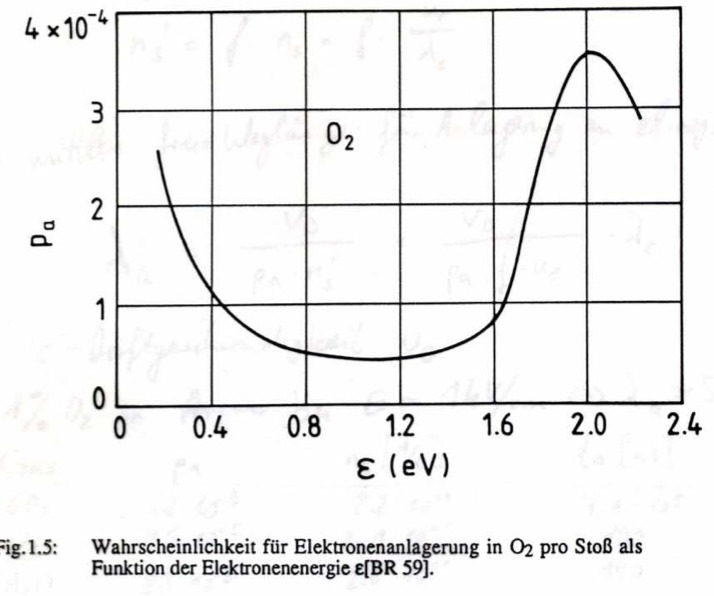
\includegraphics[width=0.5\textwidth]{Fig-03-05.jpg}
\end{figure}

With the help of the thermal velocity of the electrons 

\[u_e = \sqrt{\frac{8kT}{\pi m}}  \]

and their mean free path $\lambda_e \approx 4\cdot \lambda_{\text{Ion}}$, we obtain the number of
impacts per time interval $n_S$:

\[ n_S = \frac{u_e}{\lambda_e}  \]

and from that we can conclude, inserting the the probability of attachement $p_a$ per impact, the
mean time until attachement occurs:

\[t_a=\frac{1}{p_a\cdot n_S}  \]

If electronegative molecules are present in a gas with a share of $f$, the impact rate reduces to 

\[n_S' = f\cdot n_S = f\cdot \frac{u_e}{\lambda_e} \]

and for the drift velocity $v_D$ of the electrons, the mean free path until attachment follows with 

\[\lambda_a = \frac{v_D}{p_a\cdot n_S'}=\frac{1}{p_a\cdot f}\cdot \frac{v_D}{u_e}\cdot \lambda_e  
.\]

Example: 1\% O$_2$ in argon leads with a drift field strength of $E=1\,$keV/cm to
$\lambda_a\approx5\,$cm, which implies a loss of electrons for large drift distances.
